\documentclass{beamer}

\usepackage[brazil]{babel}
\usepackage[utf8x]{inputenc}

\usetheme{Berkeley}

\title{Segurança no padrão IEEE 802.15.4 e ZigBee}
\author{Iuri Guerra}

\begin{document}
  \frame{
	\frametitle{Departamento de Engenharia de Computação e Automação}  
	\titlepage
  }
  
  \section{Sumário}
  \frame{\tableofcontents}
  
  \section{Introdução}
  \frame{
    \frametitle{Introdução}
    \begin{itemize}
      \item Tecnologias wireless
      \begin{itemize}
	\item Vantagens e desvantagens
      \end{itemize}
    \end{itemize}
    \begin{figure}[ht!]
	\centering
	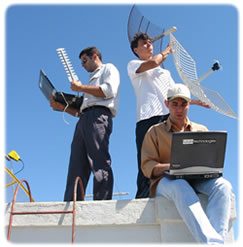
\includegraphics[width=.5\textwidth]{figuras/foto_wireless}
	\label{fig:wireless}
     \end{figure}
  }
  
  \frame{
    \frametitle{Por que se preocupar com segurança?}
    \begin{itemize}
      \item Crescimento no uso da tecnologia
      \item O meio de transmissão é o ar
      \item Maior quantidade de dados trafegando a cada dia
      \item Melhorias na tecnologia para lidar com essa quantidade dados
      \item Necessidade de garantir segurança e integridade para diversas possibilidades de aplicações
    \end{itemize}
  }

  \section{O IEEE 802.15.4}
  \frame
  {
    \frametitle{E agora, quem poderá nos defender?}
     \begin{figure}[ht!]
	\centering
	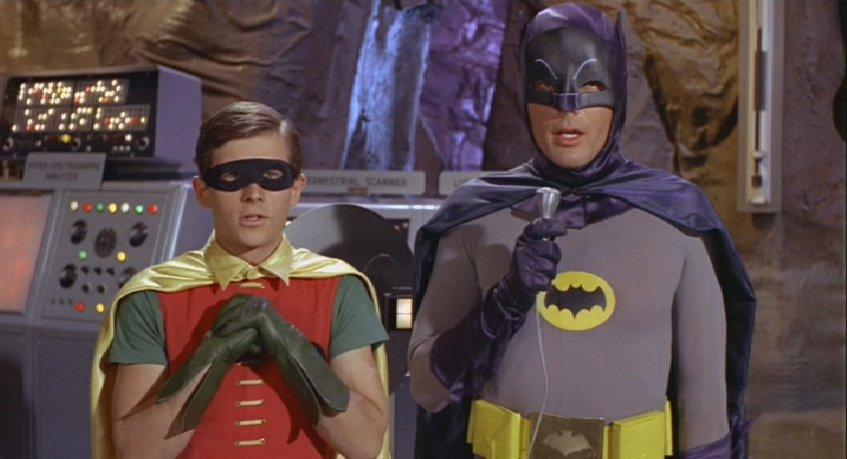
\includegraphics[width=.7\textwidth]{figuras/batmanrobin}
	\caption{IEEE 802.15.4 e Zigbee}
	\label{fig:batmanrobin}
     \end{figure}
     
  }

  \frame
  {
    \frametitle{O padrão IEEE 802.15.4}
    \begin{itemize}
      \item Criada pela IEEE e liberada em maio de 2003
      \item Especifíca a camada física e a camada MAC (Media Access Control) para dispositivos que não precisem de alta taxa de dados 
	    e que necessitem de baixa latência e baixo custo de energia
      \item É, portanto, um protocolo de pacote de dados para rede sem fio
    \end{itemize}
  }

  \frame
  {
    \frametitle{O padrão IEEE 802.15.4}
        
    \begin{figure}[ht!]
	\centering
	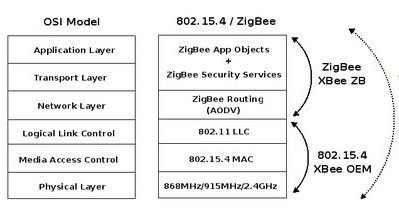
\includegraphics[width=.6\textwidth]{figuras/padrao802154}
	\label{fig:padrao}
     \end{figure}
  }

  \frame
  {
    \frametitle{Características}
    \begin{itemize}
      \item Utiliza o CSMA-CA para acesso ao meio, o mesmo do WiFi
      \item Possui estrutura sinalizadora chamada Beacon
      \item Segurança multi-camada
      \item Utiliza superframes
      \item Reconhecimento de mensagem
    \end{itemize}
  }

  \frame
  {
    \frametitle{Frequências e canais}
    27 canais distribuidos em 3 bandas
    \begin{itemize}
      \item Europa - 868.0 à 868.6 MHz (1 canal)
      \item EUUU - 902.0 à 928.0 MHz (10 canais)
      \item Resto do mundo - 2.40 à 2.48 GHz (16 canais)
    \end{itemize}
  }

  \frame
  {
    \frametitle{Taxa de dados}
    \begin{itemize}
      \item 868.0 à 868.6 MHz - 20/100/250 Kb/s
      \item 902.0 à 928.0 MHz - 40/250 Kb/s
      \item 2.40 à 2.48 GHz - 250 Kb/s
    \end{itemize}
  }

    \frame
  {
    \frametitle{Bom desenpenho contra ruído}
    \begin{itemize}
	\item Utiliza DSSS
	  \begin{itemize}
	    \item Sequência direta de espalhamento do espectro
	    \item Fornece uma densidade espectral da potência muito baixa espalhando a potência do sinal sobre uma faixa de frequência muito larga
	    \item Requer uma largura de faixa muito grande para transmitir diversos Mbits/s.
	  \end{itemize}
	\item Menos interferência de bandas utilizadas
	\item Melhoria na relação sinal/ruído no receptor
    \end{itemize}
  }

  \frame
  {
    \frametitle{Bom desenpenho contra interferências}
    \begin{itemize}
	\item CSMA-CA
	\item GTS - Garantia de slot de tempo
	\item Escaneamento de energia
	  \begin{itemize}
	    \item Energia
	    \item CCA (Carrier Sense)
	    \item CCA + Energia
	  \end{itemize}
    \end{itemize}
  }

   \frame
  {
    \frametitle{Baixo consumo}
    \begin{itemize}
	\item Sleep em 99\% do tempo
	\begin{figure}[ht!]
	  \centering
	  
\includegraphics[width=.7\textwidth]{figuras/homer}
	  \label{fig:homer}
     \end{figure}
    \end{itemize}
  }

  \frame
  {
    \frametitle{Dispositivos da rede}
    \begin{itemize}
      \item Dispositivos de Função Completa (FFD)
      \item Dispositivos de Função Reduzida (RFD)
    \end{itemize}
  }

  \frame
  {
    \frametitle{Arquitetura de transporte de dados}
    \begin{figure}[ht!]
	  \centering
	  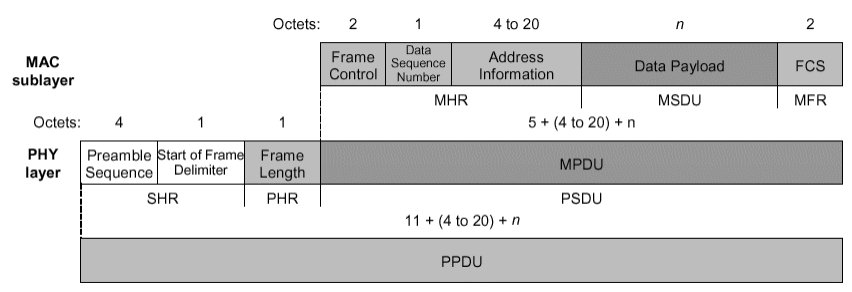
\includegraphics[width=.8\textwidth]{figuras/dataframe}
	  \caption{Dataframe}
	  \label{fig:dataframe}
    \end{figure}
  }

  \frame
  {
    \frametitle{Arquitetura de transporte de dados}
    \begin{figure}[ht!]
	  \centering
	  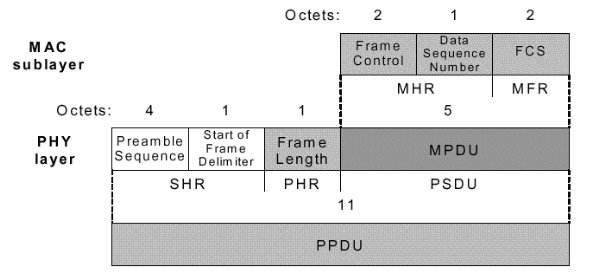
\includegraphics[width=.8\textwidth]{figuras/ackframe}
	  \caption{ACK Frame}
	  \label{fig:ackframe}
    \end{figure}
  }

  \frame
  {
    \frametitle{Arquitetura de transporte de dados}
    \begin{figure}[ht!]
	  \centering
	  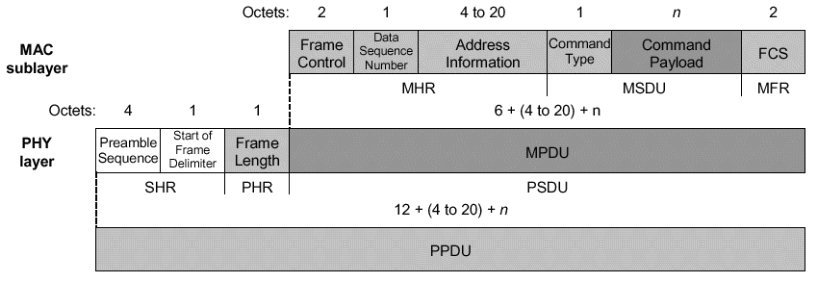
\includegraphics[width=.8\textwidth]{figuras/maccommandframe}
	  \caption{MAC Command frame}
	  \label{fig:comandframe}
    \end{figure}
  }

  \frame
  {
    \frametitle{Arquitetura de transporte de dados}
    \begin{figure}[ht!]
	  \centering
	  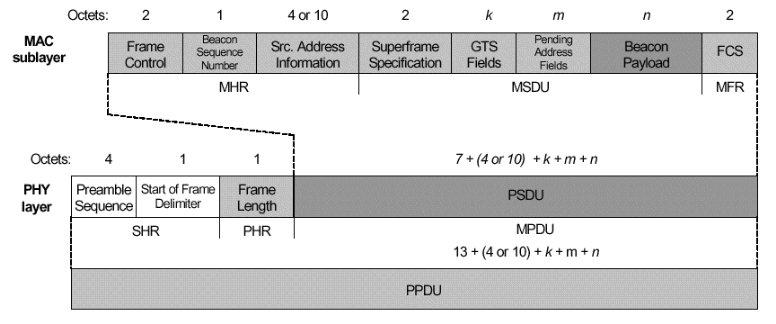
\includegraphics[width=.8\textwidth]{figuras/beaconframe}
	  \caption{Beacon frame}
	  \label{fig:beacon}
    \end{figure}
  }

    \frame
  {
    \frametitle{Arquitetura de transporte de dados}
    \begin{figure}[ht!]
	  \centering
	  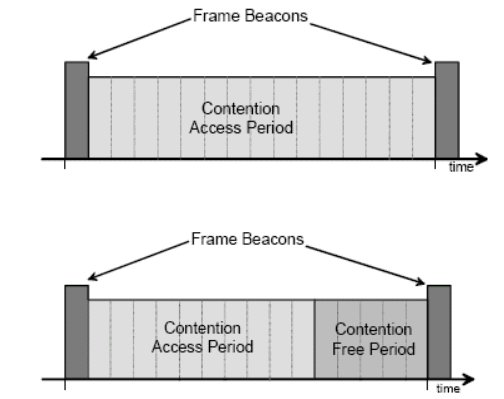
\includegraphics[width=.7\textwidth]{figuras/superframe}
	  \caption{Super Frame}
	  \label{fig:superframe}
    \end{figure}
  }

  \section{O Protocolo ZigBee}
  \frame
  {
    \frametitle{ZigBee}
    \begin{itemize}
      \item \textbf{Serviço de encriptação extra:} chaves de rede e aplicação implementam 128b de encriptação AES;
      \item \textbf{Associação e autenticação:} somente nós válidados podem ingressar na rede;
      \item \textbf{Protocolo de roteamento:} AODV, um protocolo ad hoc reativo, tem sido implementado para realizar o roteamento de dados e processo 
	    de encaminhamento para qualquer nó na rede
      \item \textbf{Serviços de aplicações:} um termo abstrato denominado "cluster" é introduzido. Cada nó pertence a um cluster pré-definido e pode 
	    obter um pré-definido número de ações. Por exemplo: o cluster do sistema de luz da casa pode realizar duas ações; ligar a luz e desligar a luz.
    \end{itemize}
  }
  
  \frame
  {
    \frametitle{Funcionamento de uma rede ZigBee}
    \begin{itemize}
      \item Coordenador (FFD)
      \item Roteador (FFD)
      \item Dispositivo final (FFD ou RFD)
    \end{itemize}
  }

    \frame
  {
    \frametitle{Topologias de rede ZigBee}
    \begin{figure}[ht!]
	  \centering
	  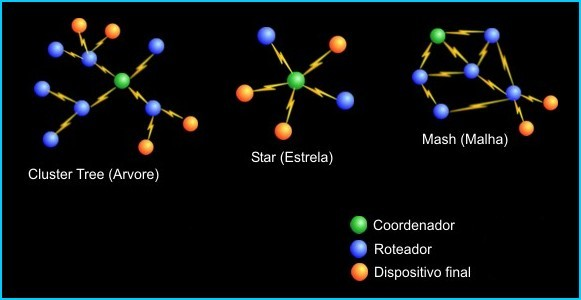
\includegraphics[width=.8\textwidth]{figuras/TopologiaZigBee}
	  \label{fig:topologias}
    \end{figure}
  }
  
    \frame
  {
    \frametitle{Funcionamento de uma rede ZigBee}
    \begin{itemize}
      \item 802.15.4 foi idealizado para ser um protocolo que estabelece comunicações pontoa-ponto com eficiência de energia.
      \item ZigBee define serviços extras (roteamento em topologia estrela, encriptação, serviços de aplicação) acima da camada 802.15.4.
      \item ZigBee cria redes semi-centralizadas aonde apenas o dispositivo final pode ficar em estado de hibernação (sleep).
    \end{itemize}
  }
  
  \section{Segurança IEEE 802.15.4}
  \frame
  {
    \frametitle{Visão geral}
    \begin{itemize}
      \item AES (Advanced Encryption Standard)
      \item Chave de 128 bits
      \item Utilizado para encriptar e validar dados
      \item Código de Integridade de Mensagem
    \end{itemize} 
  }

    \frame
  {
    \frametitle{Quadro MAC}
        \begin{figure}[ht!]
	  \centering
	  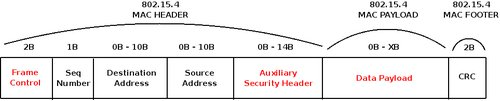
\includegraphics[width=.8\textwidth]{figuras/mac802154_0med}
	  \label{fig:mac1}
    \end{figure}
  }

  \frame
  {
    \frametitle{Quadro MAC}
    O frame de Controle de Segurança Auxiliar é habilitado somente se o subcampo de Segurança Habilitada do Frame de controle estiver ligado. Esse
    cabeçalho tem 3 campos:
    \begin{itemize}
      \item \textbf{Controle de Segurança (1B):} especifica que tipo de proteção é utilizada.
      \item \textbf{Contador de Frame (4B):} é um contador fornecido pela fonte do frame atual para proteger a mensagem contra repetição de proteção. 
	    Por esta razão cada mensagem tem uma única ID sequência representada por este campo.
      \item \textbf{Identificador de chave (0-9B):} especifica a informação necessária para saber que chave nós estamos usando com o nó que estamos 
	    nos comunicando.
    \end{itemize}
  }

    \frame
  {
    \frametitle{Quadro MAC}
        \begin{figure}[ht!]
	  \centering
	  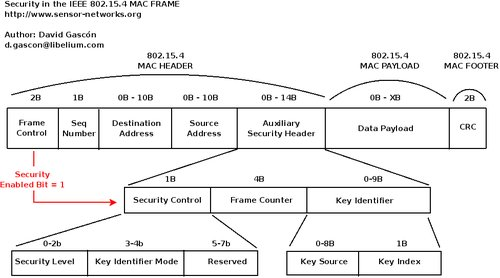
\includegraphics[width=.8\textwidth]{figuras/mac8021540med}
	  \label{fig:mac2}
    \end{figure}
  }

   \frame
  {
    \frametitle{Controle de Segurança}
   O controle de segurança é o local onde a nossa política de segurança global é configurada.
   Utilizando os 2 primeiros bits (campos de nível de segurança) escolhe-se o que será encriptado e quão longa a chave será:
   \begin{table}[htb] % [htb]-> here, top, bottom
   \centering   % tabela centralizada
   \footnotesize       % tamanho da fonte 
   \setlength{\arrayrulewidth}{2\arrayrulewidth}  % espessura da  linha
   \setlength{\belowcaptionskip}{4pt}  % espaço entre caption e tabela
   %\caption{Tabela com as respectivas chaves para o tipo de encriptação de acordo com os bits do nível de segurança}
   \begin{tabular}{|l|l|l|l|} % c=center, l=left, r=right 
      \hline
      0x00 & Sem segurança &  & DNE*, ANV**\\
      \hline
      0x01 & AES-CBC-MAC-32 & MIC-32 & DNE, AV****\\
      \hline
      0x02 & AES-CBC-MAC-64 & MIC-64 & DNE, AV\\
      \hline
      0x03 & AES-CBC-MAC-128 & MIC-128 & DNE, AV\\
      \hline
      0x04 & AES-CTR & ENC & DE***, ANV\\
      \hline
      0x05 & AES-CCM-32 & AES-CCM-32 & DE, ANV\\
      \hline
      0x06 & AES-CCM-64 & AES-CCM-64 & DE, AV\\
      \hline
      0x07 & AES-CCM-128  & AES-CCM-128 & DE, AV\\
      \hline
   \end{tabular}
   \label{tab:encriptacao}
\end{table}
* Dados não encriptados
** Autenticidade dos dados não validada
*** Dados encriptados
**** Autenticidade dos dados validada
  }

    \frame
  {
    \frametitle{Controle de Segurança - Identificador de modo de chave }
    O subcampo do modo de identificação de chave configura o tipo (implícito ou explícito)
    que a chave deve ser utilizada pelo destinatário e o remetente. Possíveis valores
    são:
    \begin{itemize}
      \item \textbf{0:} O ID da chave é implicita para o remetente e destinatário (não é especificada na
	    mensagem).
      \item \textbf{1:} O ID da chave é determinada explicitamente pelo index de chave de 1 Byte vindo
	    do campo identificador de chave e do macDefaultKeySource.
      \item \textbf{2:} O ID da chave é determinado explicitamente pelo index de chave de 1 Byte e os
	    4 Bytes da fonte de chave (Key Source).
      \item \textbf{3:} O ID da chave é determinado explicitamente pelo index de chave de 1 Byte e os
	    8 Bytes da fonte de chave (Key Source).
    \end{itemize}  
  }

  \frame
  {
    \frametitle{Payload data}
    \begin{itemize}
      \item \textbf{AES-CTR:} Todos os dados são encriptados utilizando a chave definida de 128 bits
	      e o algorítmo AES. O contador de frame configura uma única ID de mensagem, e o
	      contador de chave (key counter) no subcampo de controle de chave é utilizado pela
	      camada de aplicação se o valor máximo do frame counter é atingido.
      \item \textbf{AES-CBC-MAC:} O MAC (Código de autenticidade de mensagem) é anexado ao
	      final da carga de dados (data payload). Seu tamanho depende do nível de segurança
	      especificado no campo de política de segurança (Security Policy). O MAC é criado
	      encriptando informação do cabeçalho MAC do 802.15.4 e da carga de dados.
      \item \textbf{AES-CCM:} É a mistura dos métodos definidos anteriormente. Os subcampos correspondem
	      com o modo AES-CTR mais o subcampo extra do AES-CBC-MAC encriptado.
    \end{itemize}  
  }

  \frame
  {
    \frametitle{Lista de controle de acesso}
    Quando um nó quer enviar uma mensagem para um nó específico ou recebe um pacote,
    ele irá procurar na ACL para verificar se o nó é um irmão confiável ou não. Se for, o nó
    utilizará o dado contido na coluna específica para aplicar as medidas de segurança. Caso
    o nó não esteja na lista ou sua mensagem é rejeitada ou um processo de autenticação se
    dará início.  
  }

  \section{Segurança ZigBee}
  \frame
  {
    \frametitle{Tipos de chave}
      \begin{itemize}
       \item \textbf{Master Keys:} São pré-instaladas em cada nó. Sua função é manter confidencial
	  a troca de Chaves de Link entre dois nós no Processo de Estabelecimento de
	  Chave (SKKE).
	\item \textbf{Chaves de Link:} São únicas entre cada par de nós. Essas chaves são gerenciadas
	  pelo nível de aplicação. São utilizadas para encriptar toda a informação entre cada
	  dois dispositivos, por essa razão mais recursos de memória são necessários em cada
	  dispositivo. Geralmente essa chave não constuma ser usada.
      \end{itemize}
  }

  \frame
  {
    \frametitle{Tipos de chave}
      \begin{itemize}
       \item \textbf{Chaves de Rede:} É uma chave única de 128 bits compartilhada ao longo dos dispositivos
na rede. É gerado por um centro de confiança e re-gerada em diferentes
intervalos. Casa nó precisa pegar sua chave de rede para ingressar em uma rede.
Uma vez que o centro de confiança decida mudar a chave de rede, a nova chave é
espalhada na rede utilizando a antiga chave de rede. Uma vez que essa nova chave
é atualizada em um dispositivo, seu contador de frame é inicializado em zero. Este
centro de confiança é normalmente o coordenador da rede, entretanto, pode ser que
seja um dispositivo dedicado. Ele tem apenas que autenticar e validar cada dispositivo
que tenta entrar na rede.
      \end{itemize}
  }

    \frame
  {
    \frametitle{Política de segurança}
      \begin{itemize}
       \item Modo comercial - compartilha chaves master e link, requer mais recurso de memória e oferece um modelo centralizado
       \item Modo residencial - compartilha chave de rede, ideal para rede de sensores sem fio
      \end{itemize}
  }

  \section{Conclusão}
  \frame
  {
    \frametitle{Considerações finais}
      \begin{itemize}
       \item Vale a pena?
       \item Quanto custa?
      \end{itemize}
  }
  
\end{document}
